\documentclass[10pt,a4paper]{article}
\usepackage[utf8]{inputenc}
\usepackage[T1]{fontenc}
\IfFileExists{lmodern.sty}{\usepackage{lmodern}}{}
\usepackage[margin=1.8cm]{geometry}
\usepackage{amsmath,graphicx,booktabs,xcolor,enumitem}
\usepackage[most]{tcolorbox}
\graphicspath{{figures/}}
\setlist{itemsep=1pt,topsep=2pt,leftmargin=*}
\pagestyle{empty}
\newtcolorbox{qbox}[1][Questions]{colback=orange!8,colframe=orange!75!black,fonttitle=\bfseries,title={#1},
  left=4pt,right=4pt,top=2pt,bottom=2pt}
\newtcolorbox{kbox}[1][Result]{colback=blue!5,colframe=blue!60!black,fonttitle=\bfseries,title={#1},
  left=4pt,right=4pt,top=2pt,bottom=2pt}
\newcommand{\sub}[1]{\par\smallskip\noindent\textbf{#1}\par}

\begin{document}
\begin{center}
{\Large\bfseries Mamba in 3D and 4D Gaussian Splatting --- Progress Brief}\\[2pt]
Muhammad Hussain Qureshi (MSDS25010) \quad·\quad Advisor: Dr.\ Ali Murtaza \quad·\quad 15 November 2026\\
Code and results: \texttt{github.com/muhammadhussainqureshi/thesis-gs} (\texttt{results/2026-11-15\_mamba})
\end{center}

\section*{1.\ Mamba on 3D Gaussians (inverse scattering)}
\sub{What I did, and how (PointMamba approach)}
\begin{itemize}
\item Treated the Gaussians of a volume as a \textbf{point cloud}, as in PointMamba (Liang et al., NeurIPS 2024):
farthest-point-sampled key points $\to$ patches of nearby Gaussians $\to$ one token per patch.
\item Ordered the tokens along \textbf{Hilbert and Trans-Hilbert} space-filling curves (with PointMamba's order
indicator), ran \textbf{Mamba blocks}, and gave every Gaussian a correction from its patch context.
\item Fitted per volume with the physics loss, on top of our best model (bounded, grid-initialised Gaussians), on the
\textbf{true 3D Born model} (real BBBC024 nuclei) and on 10 2D cells. Controls: per-Gaussian MLP (no neighbours) and
Mamba over a random order. New code: parallel Mamba scan, Hilbert serialisation, PointMamba encoder.
\end{itemize}

\sub{Results (PSNR dB, true 3D model, real nuclei, 3 volumes)}
\begin{center}
\begin{tabular}{lcccc}
\toprule
 & Parameters & 360 rec. & 180 rec. & 60 rec. \\
\midrule
Gaussians + \textbf{PointMamba} & 60k + 88k & \textbf{32.9} & 31.3 & 26.4 \\
Gaussians, no network & 60k & 32.8 & \textbf{31.4} & \textbf{26.7} \\
Voxel grid (same loss) & 524k & 32.5 & 30.5 & 25.6 \\
\bottomrule
\end{tabular}
\end{center}
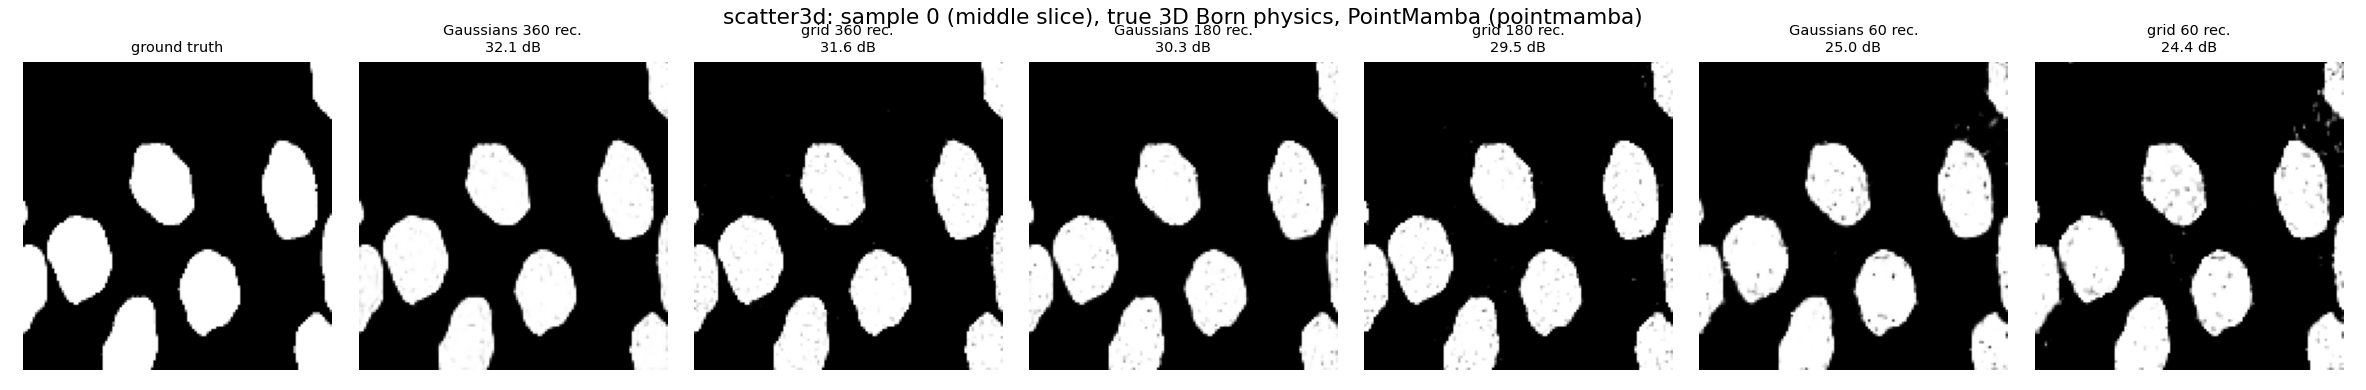
\includegraphics[width=\linewidth]{born3d_pointmamba.png}
\begin{kbox}[What it shows]
\begin{itemize}
\item PointMamba runs on 3D Gaussians and \textbf{beats the voxel grid on every volume} (+0.4 to +0.8\,dB) with
$\sim$3.5$\times$ fewer parameters, but it is \textbf{equal to the Gaussians without a network} ($\pm$0.3\,dB; in
2D all variants within $\pm$0.1\,dB).
\item Reason: Mamba only adds corrections to Gaussians that are themselves free, so it adds no constraint. To act as a
prior, Mamba must \emph{generate} the Gaussians, or be \emph{trained across volumes} (as PointMamba is pre-trained).
\end{itemize}
\end{kbox}

\newpage
\section*{2.\ Improving Mamba in 4D Gaussians (Navier--Stokes)}
\sub{What I did, and how}
\begin{itemize}
\item 4D Gaussians: canonical Gaussians + a deformation network that moves them over time (21 frames, $Re=200$).
\item \textbf{Mamba} reads each Gaussian's trajectory over time; improved with a \textbf{temporal smoothness} term, one
network pass per step for data and smoothness (about 2$\times$ faster), and tested on \textbf{5 flows} (was 3).
\item New: \textbf{space--time Mamba} (adds a PointMamba spatial scan across Gaussians in every frame).
\item Only 10\% of pixels observed; 5 frames never observed (tested).
\end{itemize}

\sub{Results (PSNR dB on unseen frames, 10\% observed)}
\noindent\begin{minipage}[t]{0.46\linewidth}\vspace{0pt}
\begin{tabular}{lc}
\toprule
Model & PSNR \\
\midrule
MLP (4DGS-style), 5 flows & 23.1 $\pm$ 1.4 \\
Mamba, first version, 3 flows & 23.1 \\
Mamba + smoothness, 3 flows & 25.4 \\
\textbf{Mamba (current), 5 flows} & \textbf{25.9 $\pm$ 1.1} \\
Space--time Mamba, 5 flows & 25.8 $\pm$ 1.3 \\
\bottomrule
\end{tabular}
\begin{kbox}[What it shows]
\begin{itemize}
\item Mamba improved from 23.1 to \textbf{25.9\,dB}.
\item It beats the MLP on \textbf{all 5 flows}, by \textbf{+2.8 $\pm$ 0.9\,dB}.
\item The MLP leaves streaks; Mamba stays coherent.
\item The spatial scan adds nothing ($-0.2$\,dB).
\end{itemize}
\end{kbox}
\end{minipage}\hfill
\begin{minipage}[t]{0.51\linewidth}\vspace{0pt}
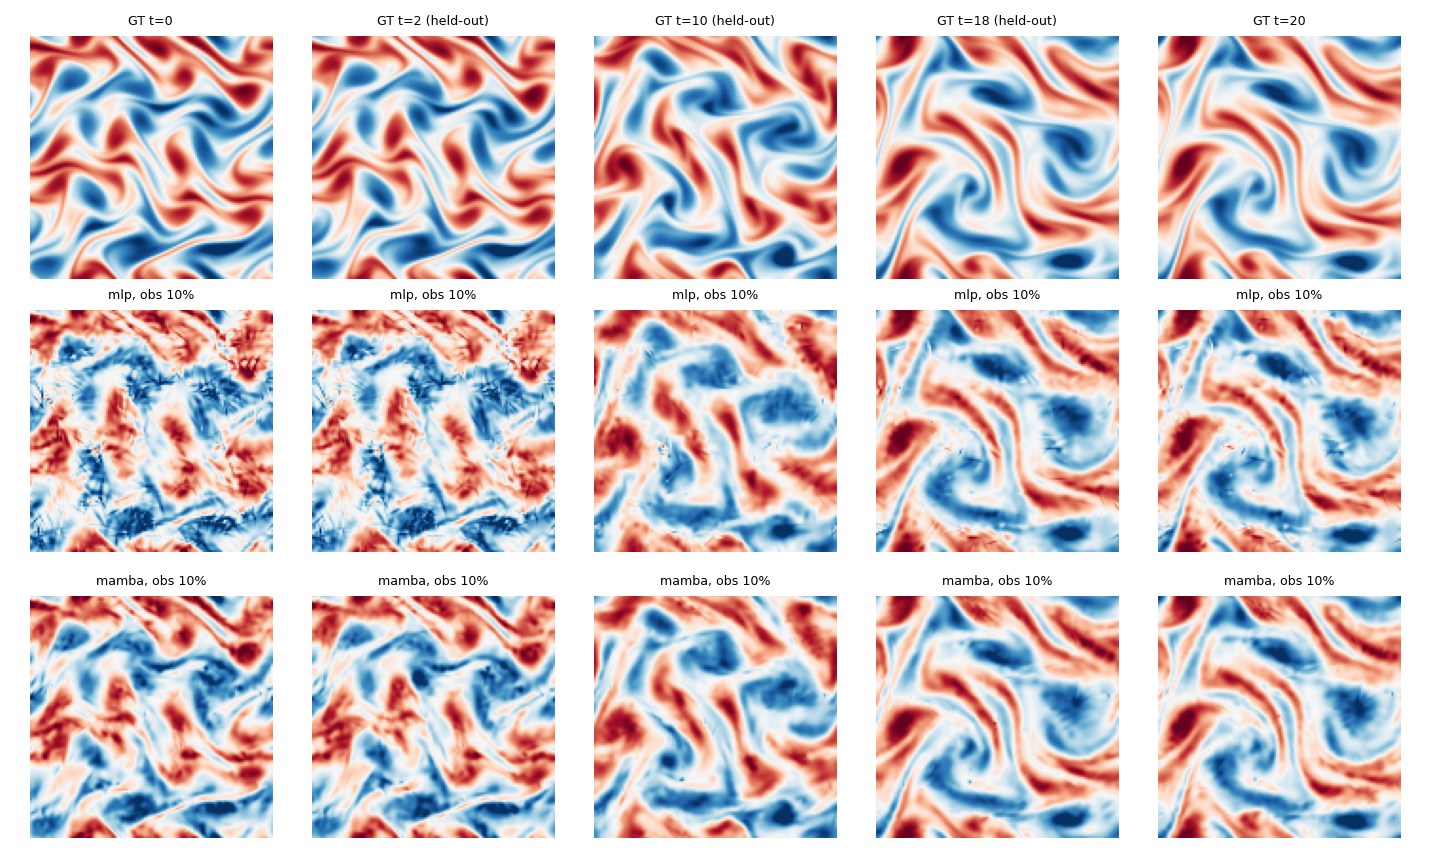
\includegraphics[width=\linewidth]{ns4d_mlp_vs_mamba.png}\\
{\footnotesize Flow 0. Rows: truth, MLP, Mamba (10\% observed). Frames 2, 10, 18 never observed.}
\end{minipage}

\medskip
\begin{qbox}
\begin{enumerate}
\item \textbf{3D:} next step for Mamba --- (a) Mamba \emph{generates} the Gaussians (one more run), or (b) a PointMamba
network trained across volumes (larger, Thesis II)? Or is the current 3D Mamba result enough for Thesis I?
\item \textbf{4D:} is Mamba with temporal smoothness (+2.8\,dB over the MLP) sufficient for Thesis I?
\item Can I now freeze experiments and finish the thesis document, slides and poster?
\end{enumerate}
\end{qbox}
\end{document}
